\chapter{Résultats et discussion}

\section{Introduction}

Après avoir présenté la méthodologie de construction du corpus parallèle ruund--français ainsi que le développement du système de traduction automatique basé sur les modèles neuronaux, il est indispensable d'évaluer les performances obtenues afin d'apprécier la capacité de ces modèles à produire des traductions de qualité. L'évaluation constitue une étape essentielle dans le développement d'un système de traduction automatique, puisqu'elle permet de mesurer objectivement les performances des modèles, d'identifier leurs forces et leurs limites, et de déterminer l'approche la plus adaptée au contexte des \ac{LFR}.

Ce chapitre présente les résultats obtenus à l'issue du processus de \textit{fine-tuning} des différents modèles de traduction. Les performances sont d'abord analysées à l'aide de métriques d'évaluation automatiques, qui permettent d'estimer la proximité des traductions générées avec les traductions de référence. Cette évaluation est ensuite complétée par une analyse qualitative reposant sur une évaluation humaine. Cette double approche permet d'apprécier non seulement la qualité lexicale et syntaxique des traductions, mais également leur fidélité sémantique et leur fluidité.

Enfin, une discussion critique des résultats est proposée afin d'interpréter les performances observées en tenant compte des caractéristiques du corpus parallèle, des spécificités linguistiques du ruund. Cette analyse permet de mettre en évidence les principaux facteurs ayant influencé les performances du système développé, d'identifier les limites de l'étude et de dégager des perspectives d'amélioration pour les travaux futurs.

\section{Résultats quantitatifs}
\label{sec:resultats_quantitatifs}

L'évaluation quantitative des modèles de traduction automatique a été réalisée à l'aide de deux métriques largement utilisées dans le domaine de la \textbf{\ac{TAN}} : le score \textbf{\ac{BLEU}} et le score \textbf{\ac{chrF}}. Le score \ac{BLEU} mesure le degré de correspondance entre la traduction générée et la traduction de référence à partir des \textit{n-grammes} de mots, tandis que le score \ac{chrF} repose sur les \textit{n-grammes} de caractères, ce qui le rend particulièrement adapté à l'évaluation des langues présentant une forte richesse morphologique ou disposant de ressources limitées. En complément, le temps d'entraînement de chaque modèle a été relevé afin d'apprécier le coût computationnel associé au processus de \textit{fine-tuning}.

\subsection{Présentation des résultats des métriques automatiques}
\label{subsec:resultats_metriques}

Les performances obtenues par les trois modèles étudiés --- \ac{mBART}-50, \ac{NLLB}-200-distilled-600M et \ac{MarianMT} --- ont été mesurées pour les deux directions de traduction, à savoir du ruund vers le français et du français vers le ruund.

Les résultats montrent des différences significatives entre les modèles évalués. Pour les deux directions de traduction, le modèle \ac{NLLB}-200-distilled-600M obtient systématiquement les meilleurs scores \ac{BLEU} et \ac{chrF}. Le modèle \ac{mBART}-50 se situe en deuxième position, avec des performances satisfaisantes bien qu'inférieures à celles de \ac{NLLB}-200-distilled-600M, tandis que \ac{MarianMT} affiche les performances les plus faibles, en particulier pour la direction français--ruund.

Concernant le temps d'entraînement, les trois modèles présentent des durées relativement proches, comprises entre environ neuf et quinze minutes selon la direction de traduction. Malgré un nombre de paramètres comparable à celui de \ac{mBART}-50, le modèle \ac{NLLB}-200-distilled-600M présente un temps d'entraînement légèrement inférieur tout en offrant des performances nettement supérieures.

Le Tableau~\ref{tab:resultats_metriques} présente les résultats détaillés des métriques automatiques pour les trois modèles.
\begin{table}[H]
\centering
\renewcommand{\arraystretch}{1.4}
\rowcolors{2}{gray!10}{white}
\begin{tabular}{p{4cm}p{4cm}ccc}
\toprule
\textbf{Modèle} & \textbf{Direction} & \textbf{\ac{BLEU}} & \textbf{\ac{chrF}} & \textbf{Temps d'entraînement} \\
\midrule
\ac{mBART}-50 & Ruund $\rightarrow$ Français & 20,84 & 43,38 & 12~min~47~s \\
\ac{mBART}-50 & Français $\rightarrow$ Ruund & 25,23 & 51,92 & 14~min~40~s \\
\ac{NLLB}-200-distilled-600M & Ruund $\rightarrow$ Français & \textbf{37,55} & \textbf{57,25} & 12~min~30~s \\
\ac{NLLB}-200-distilled-600M & Français $\rightarrow$ Ruund & \textbf{26,02} & \textbf{53,95} & 13~min~27~s \\
\ac{MarianMT} & Ruund $\rightarrow$ Français & 15,56 & 40,24 & 14~min~58~s \\
\ac{MarianMT} & Français $\rightarrow$ Ruund & 10,64 & 36,79 & 8~min~48~s \\
\bottomrule
\end{tabular}
\caption{Performances des modèles selon les scores \ac{BLEU} et \ac{chrF}}
\label{tab:resultats_metriques}
\end{table}

\subsection{Analyse comparative des performances des modèles}
\label{subsec:analyse_comparative}

L'analyse met en évidence l'intérêt des modèles multilingues de grande capacité pour les \textbf{\ac{LFR}}. Avec environ 600 millions de paramètres, \ac{mBART}-50 et \ac{NLLB}-200-distilled-600M disposent d'une capacité de représentation largement supérieure à celle de \ac{MarianMT}, qui compte environ 60 millions de paramètres. Cette différence de capacité favorise l'apprentissage de représentations linguistiques plus riches et améliore la généralisation lors du \textit{fine-tuning} sur un corpus de taille limitée.

Les performances plus faibles de \ac{MarianMT} peuvent également être attribuées au fait que le modèle d'origine, \texttt{Helsinki-NLP/opus-mt-en-fr}, n'a pas été initialement conçu pour prendre en charge le ruund. Son adaptation au moyen de l'ajout du jeton de langue \textit{ruu\_CM} et d'un \textit{fine-tuning} sur le corpus parallèle a permis d'étendre ses capacités à cette langue, mais les résultats montrent que cette adaptation reste moins efficace que celle des modèles multilingues préentraînés sur un grand nombre de langues.

Le corpus parallèle construit dans le cadre de cette étude comprend une taille initiale de 8~431 paires de phrases, réparties en 6~492 exemples d'entraînement, 812 exemples de validation et 812 exemples de test. Malgré cette quantité relativement modeste au regard des standards actuels de la \ac{TAN}, les résultats obtenus, en particulier par le modèle \ac{NLLB}-200-distilled-600M, montrent qu'un \textit{fine-tuning} de modèles multilingues préentraînés constitue une approche pertinente pour le développement de systèmes de traduction destinés aux \ac{LFR}. Les connaissances linguistiques acquises lors du préentraînement permettent ainsi de compenser en partie la rareté des données disponibles et d'améliorer la qualité des traductions produites.

Ces résultats quantitatifs constituent une première indication des performances des différents modèles. Toutefois, les métriques automatiques ne permettent pas, à elles seules, d'apprécier pleinement la qualité des traductions générées. Une analyse qualitative complétée par une évaluation humaine est donc nécessaire afin d'examiner plus finement la fidélité sémantique, la fluidité et l'acceptabilité linguistique des traductions produites.

\subsection{Analyse de la convergence des modèles}
\label{subsec:convergence_modeles}

L'analyse des courbes d'entraînement complète l'évaluation par les métriques automatiques en permettant d'examiner la vitesse d'apprentissage, la stabilité de l'entraînement et la capacité de généralisation des trois modèles étudiés, à partir de l'évolution de la \textbf{perte d'entraînement}, de la \textbf{perte de validation} et des scores \ac{BLEU}/\ac{chrF} au fil des époques.

Le modèle \ac{NLLB}-200-distilled-600M présente la convergence la plus régulière. Pour les deux directions de traduction, les pertes d'entraînement et de validation diminuent de façon continue sur les quinze époques, tandis que les scores \ac{BLEU} et \ac{chrF} progressent jusqu'à atteindre un plateau en fin d'entraînement. L'écart limité entre les deux courbes de perte indique une bonne capacité de généralisation, sans signe marqué de \textbf{surapprentissage} (\textit{overfitting}).

Les Figures \ref{fig:nllb_convergence_ruu_fr} et \ref{fig:nllb_convergence_fr_ruu} illustrent l'évolution de la perte et des métriques automatiques pour le modèle \ac{NLLB}-200-distilled-600M en fonction des époques.
\begin{figure}[H]
    \centering
    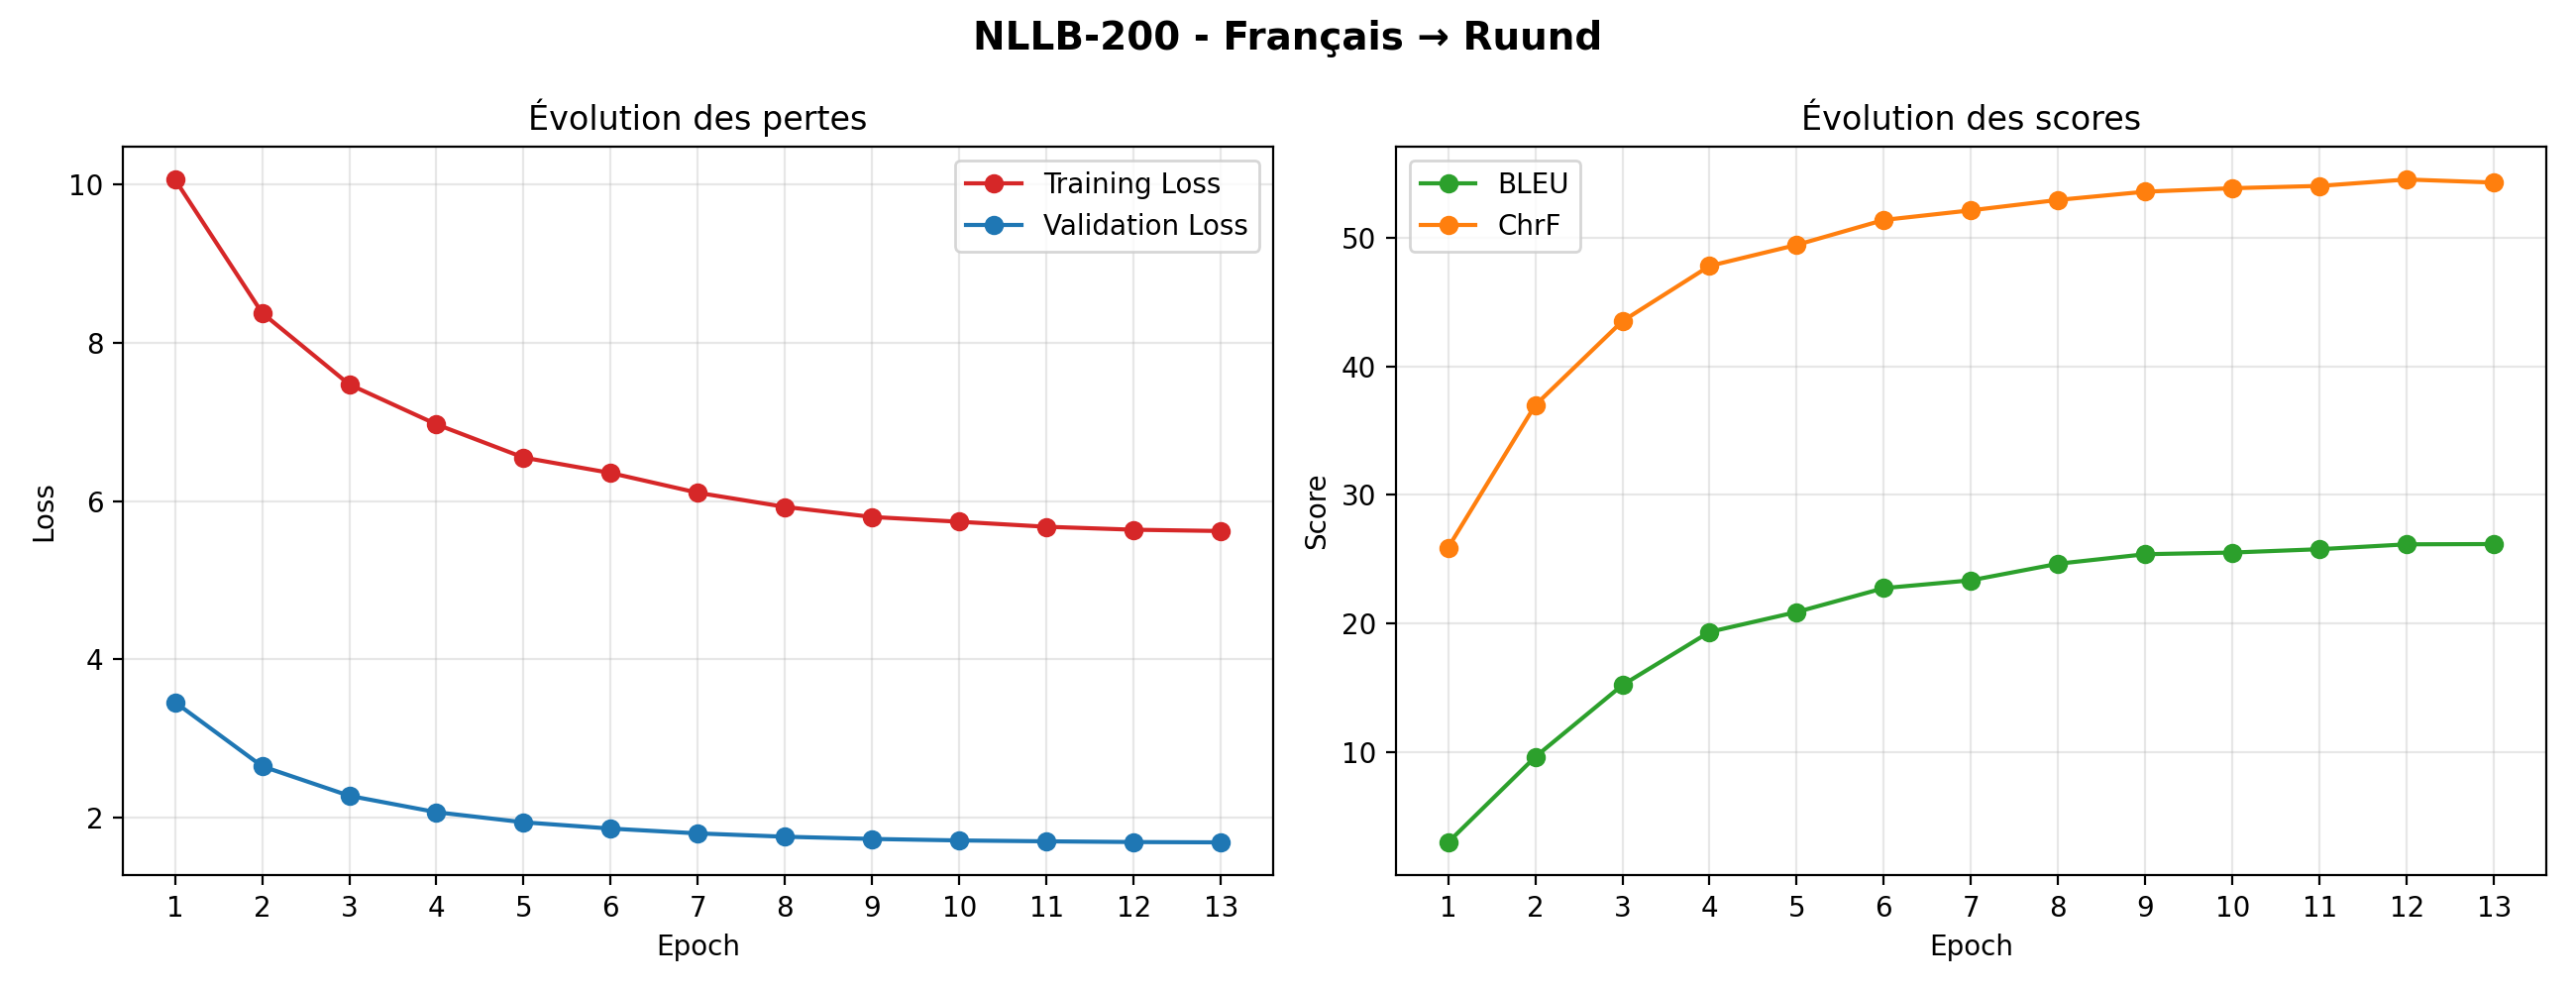
\includegraphics[width=1\textwidth]{Images/nllb_fr_ruund.png}
    \caption[Courbes d'entraînement NLLB-200-distilled-600M - Français $\rightarrow$ Ruund]{Courbes d'entraînement NLLB-200-distilled-600M - Français $\rightarrow$ Ruund}
    \label{fig:nllb_convergence_fr_ruu}
\end{figure}

\begin{figure}[H]
    \centering
    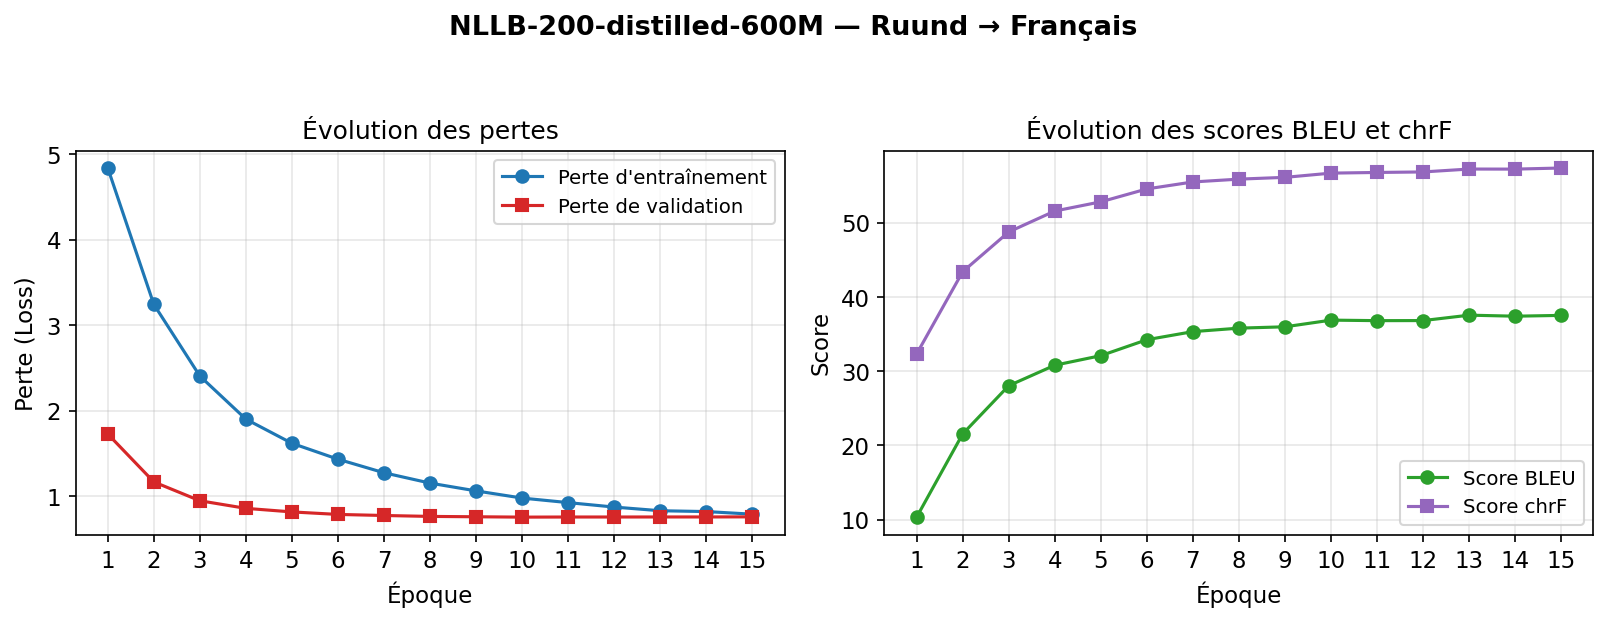
\includegraphics[width=1\textwidth]{Images/nllb_ruund_fr.png}
    \caption[Courbes d'entraînement NLLB-200-distilled-600M - Ruund $\rightarrow$ Français]{Courbes d'entraînement NLLB-200-distilled-600M - Ruund $\rightarrow$ Français}
    \label{fig:nllb_convergence_ruu_fr}
\end{figure}

Le modèle \ac{mBART}-50 converge plus rapidement sur les premières époques, avec les gains les plus importants en \ac{BLEU} et \ac{chrF} observés entre la deuxième et la quatrième époque. Au-delà de cette phase, la perte de validation augmente alors que la perte d'entraînement continue de diminuer, ce qui traduit un début de surapprentissage. Les scores \ac{BLEU} et \ac{chrF} conservent néanmoins une légère progression jusqu'à la dixième époque, sans être affectés par cette divergence des pertes.

Les Figures \ref{fig:mbart_convergence_fr_ruu} et \ref{fig:mbart_convergence_ruu_fr} illustrent l'évolution de la perte et des métriques automatiques pour le modèle \ac{mBART}-50 en fonction des époques.
\begin{figure}[H]
    \centering
    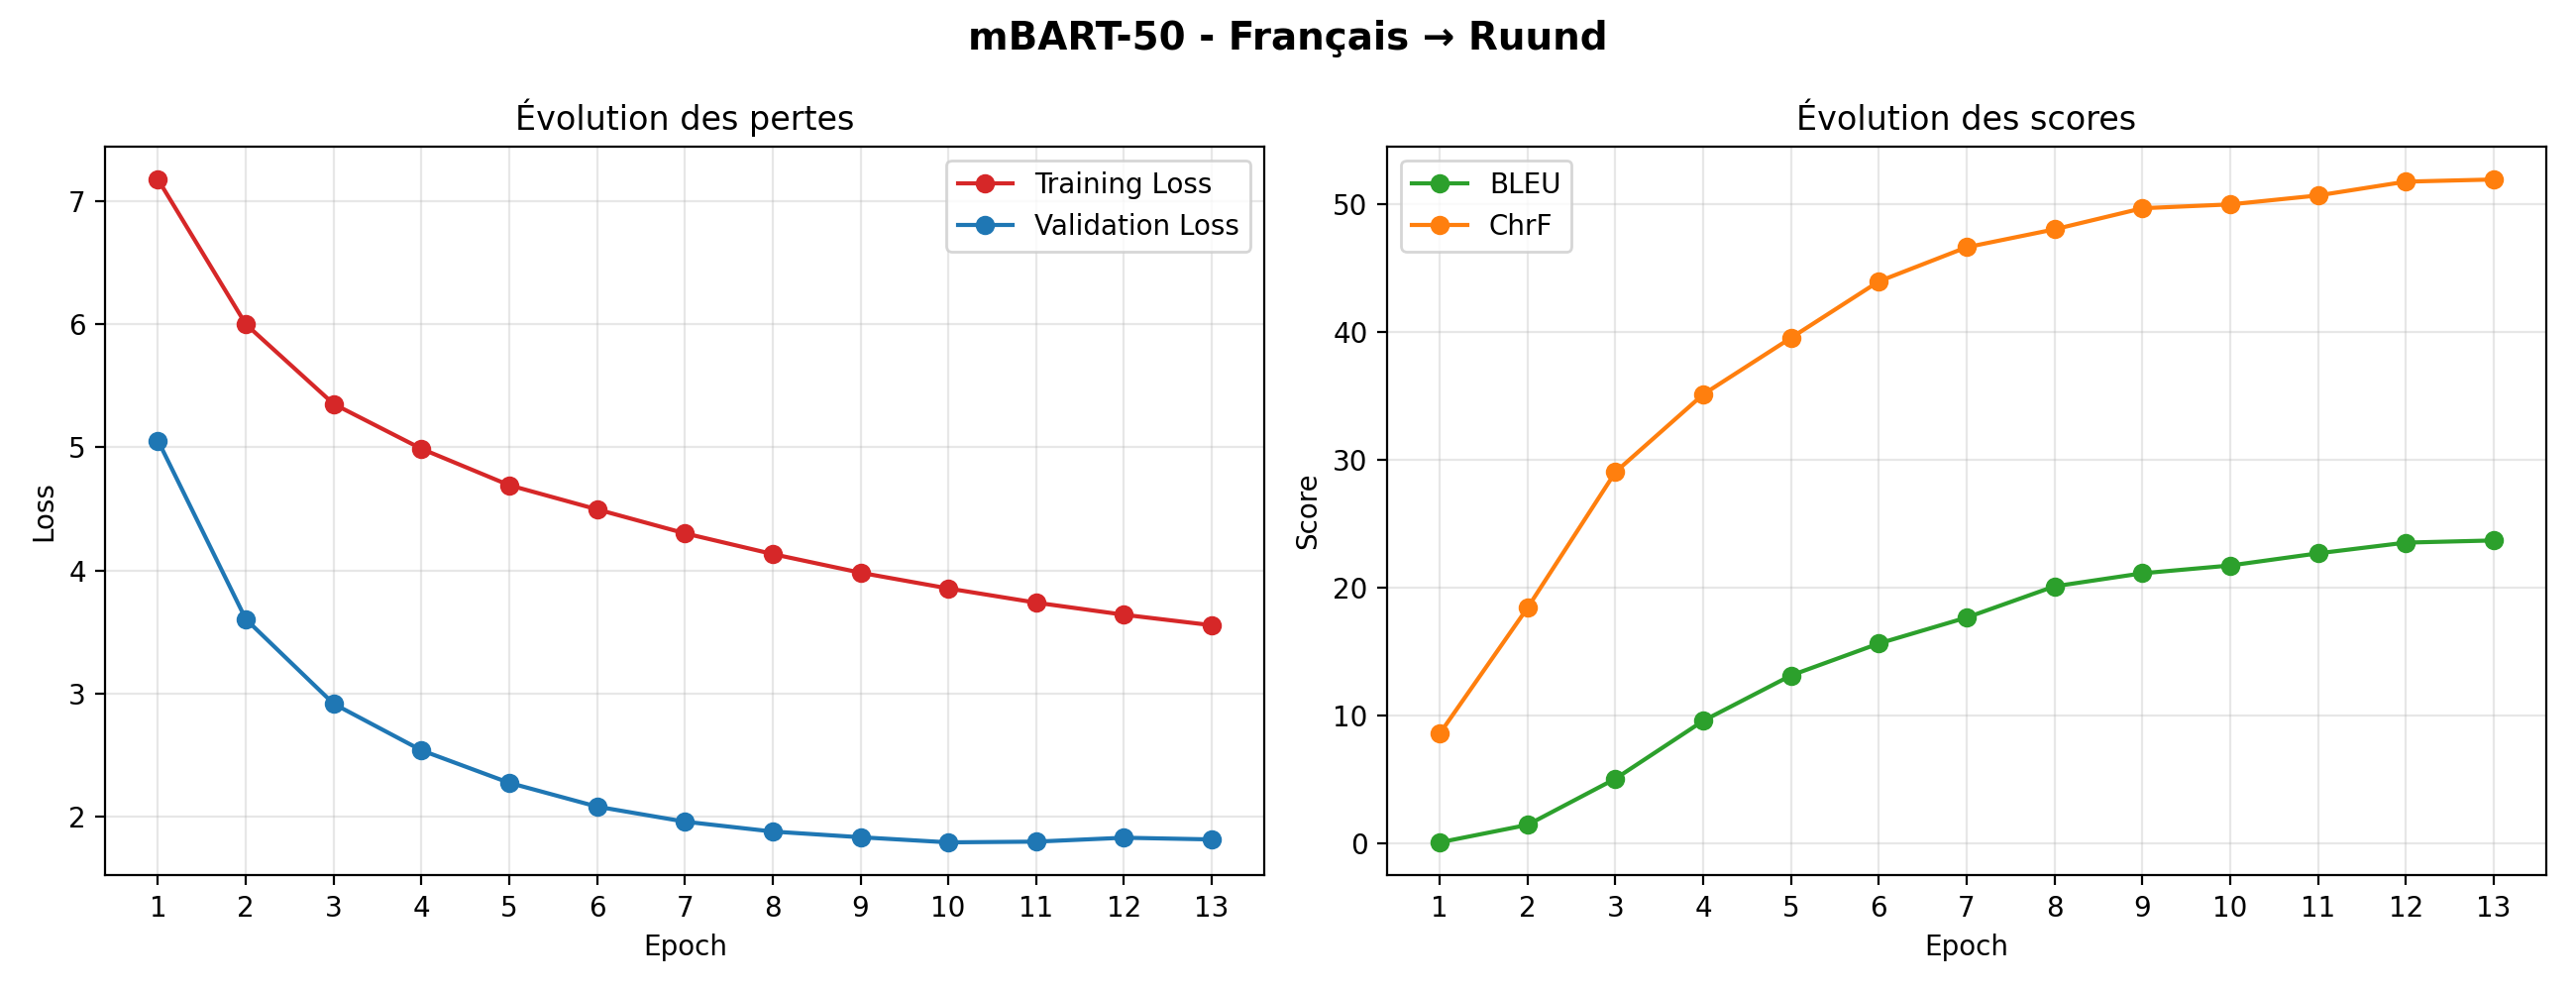
\includegraphics[width=1\textwidth]{Images/mbart_fr_ruund.png}
    \caption[Courbes d'entraînement mBART-50 - Français $\rightarrow$ Ruund]{Courbes d'entraînement mBART-50 - Français $\rightarrow$ Ruund}
    \label{fig:mbart_convergence_fr_ruu}
\end{figure}

\begin{figure}[H]
    \centering
    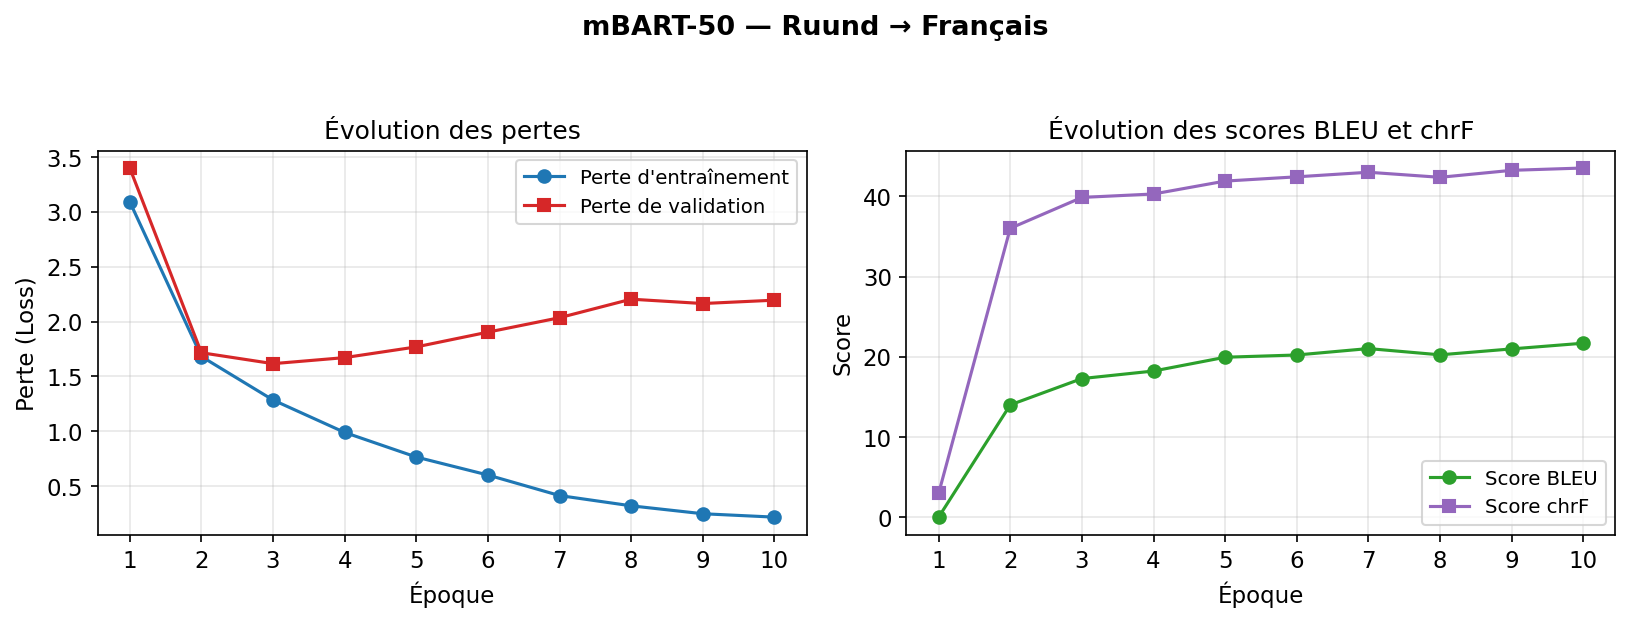
\includegraphics[width=1\textwidth]{Images/mbart_ruund_fr.png}
    \caption[Courbes d'entraînement mBART-50 - Ruund $\rightarrow$ Français]{Courbes d'entraînement mBART-50 - Ruund $\rightarrow$ Français}
    \label{fig:mbart_convergence_ruu_fr}
\end{figure}

Le modèle \ac{MarianMT} affiche une diminution régulière et stable des deux pertes, sans augmentation notable de la perte de validation. Les scores \ac{BLEU} et \ac{chrF} progressent de manière constante mais avec des gains décroissants au fil des époques, révélant une convergence vers un optimum local à un niveau de performance inférieur à celui des deux modèles multilingues.

Les Figures \ref{fig:marianmt_convergence_fr_ruu} et \ref{fig:marianmt_convergence_ruu_fr} illustrent l'évolution de la perte et des métriques automatiques pour le modèle \ac{MarianMT} en fonction des époques.
\begin{figure}[H]
    \centering
    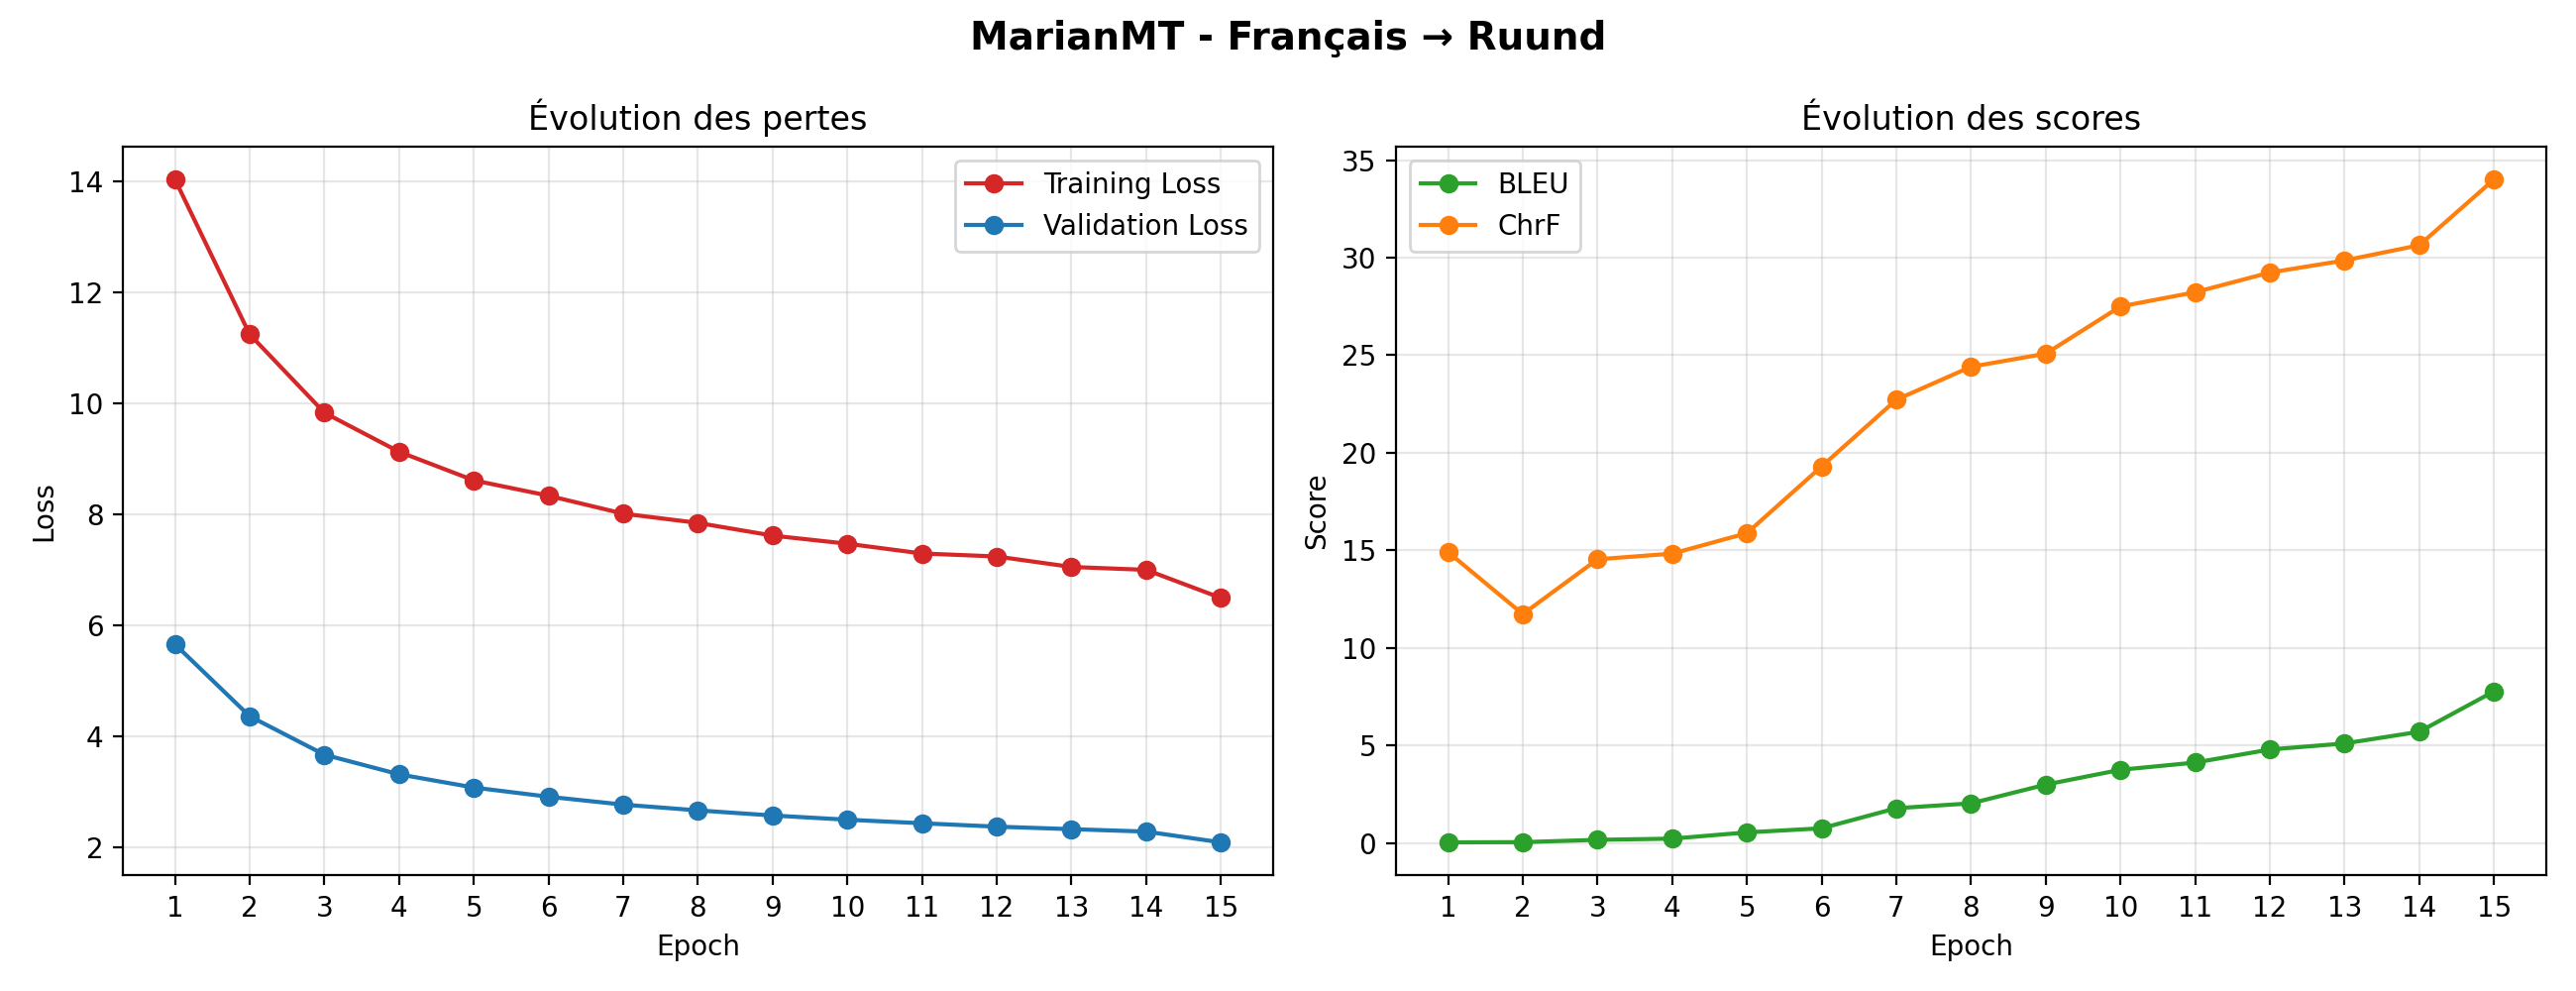
\includegraphics[width=1\textwidth]{Images/marianmt_fr_ruund.png}
    \caption[Courbes d'entraînement MarianMT - Français $\rightarrow$ Ruund]{Courbes d'entraînement MarianMT - Français $\rightarrow$ Ruund}
    \label{fig:marianmt_convergence_fr_ruu}
\end{figure}

\begin{figure}[H]
    \centering
    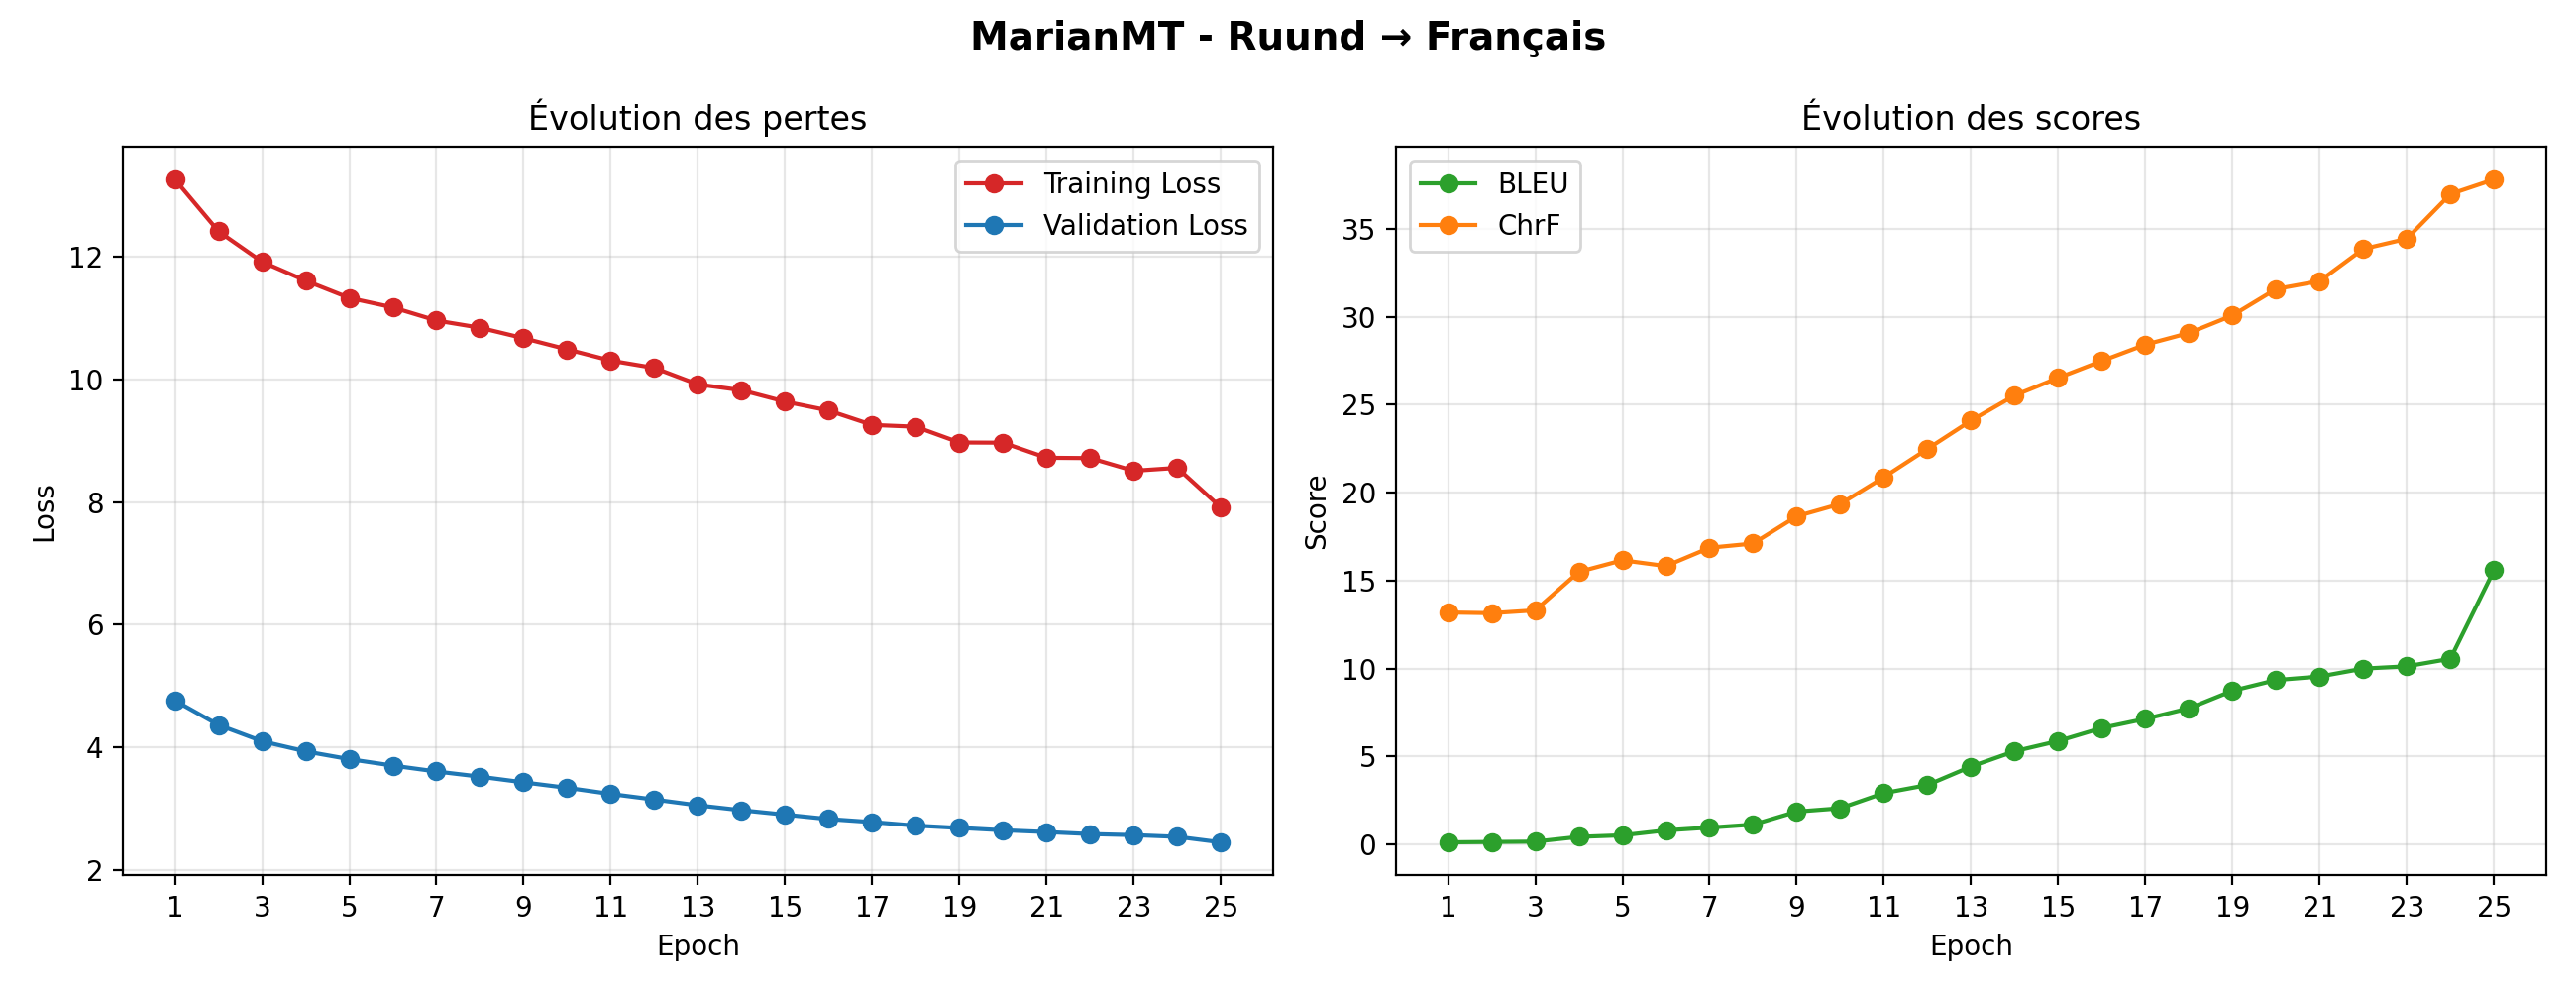
\includegraphics[width=1\textwidth]{Images/marianmt_ruund_fr.png}
    \caption[Courbes d'entraînement MarianMT - Ruund $\rightarrow$ Français]{Courbes d'entraînement MarianMT - Ruund $\rightarrow$ Français}
    \label{fig:marianmt_convergence_ruu_fr}
\end{figure}

Ces observations corroborent les résultats obtenus par les métriques automatiques (Section~\ref{subsec:resultats_metriques}) : \ac{NLLB}-200-distilled-600M combine les meilleures performances et la convergence la plus stable ; \ac{mBART}-50 apprend rapidement mais présente des signes de surapprentissage ; \ac{MarianMT} converge de façon stable sans atteindre un niveau de performance comparable. Ces résultats confirment l'intérêt des modèles multilingues préentraînés de grande capacité pour la \ac{TAN} appliquée aux \ac{LFR} telles que le ruund.

\section{Évaluation qualitative des traductions}
\subsection{Analyse d'exemples de traduction}
\subsubsection{Analyse qualitative des traductions hors contexte religieux}

Le Tableau~\ref{tab:exempletraduction} présente quelques exemples de traductions générées par les trois modèles dans les directions Français $\rightarrow$ Ruund et Ruund $\rightarrow$ Français. Les exemples retenus couvrent des textes variés, principalement hors contexte religieux, tout en incluant quelques extraits du domaine religieux\begin{landscape}
\begingroup
\renewcommand{\arraystretch}{1.4}
\small
\rowcolors{2}{gray!10}{white}
\begin{longtable}{p{4.5cm}p{4.5cm}p{4.5cm}p{4.5cm}p{4.5cm}}
\toprule
\textbf{Source} & \textbf{Référence} & \textbf{\ac{NLLB}-200} & \textbf{\ac{mBART}-50} & \textbf{\ac{MarianMT}} \\
\midrule
\endfirsthead
\endhead

\bottomrule
\endfoot

\bottomrule
\endlastfoot
Bonjour, je suis Uriel et je viens de Kolwezi. J'aime les femmes comme le Christ a aimé l'Église. J'ai remarqué que pour avoir de l'argent, il faut travailler, ce qui est difficile à faire, sachant que la majorité des personnes dans le pays sont au chômage. Je vous remercie, que le Seigneur vous bénisse et multiplie le poisson dans votre génération. & Walankan, dijine dam uriel ,nid mu Kolwezi, nikatine emband mud kristu mukatinaye chikumb chend cha nzamb ,nimen kwikal ni nfalang ifandin kusal mudum,ikasken kwihisal,mutap enchu avud mwi ngand kadap ni mudum , nikujikitishinan  ni nzamb akuyukishan ,avudish enshi mu chipuk Chen & mwalany, am nidi uriel wa ku kolwezi. nikatil amband mudi mukatilay kristu in chikumbu cha nzamb. natesha anch, chakwel ukwet nfalang, ufanyidin kusal mudimu, mulong antu avud a mu mangand minam akwet mudimu. nakushimanany, chifanyidin nzamb akuyukishany ni kupan ansh avud mu chisak chen. & nakwitiyany, am uriel, nidiokil ku musumb wa kolowezi. nikat ambwez ambach pa ambweny, nikat kukat ambwez chidi chom chamwamu, mulong kristu watutazuka kand in chikumbu cha nzamb. nova kudi en anch, chifanyidin nsalejetu akwinkishany yiyukish yau ni kupalangan mu yisak yen yau. & am nikat kulembil kudiokal ku musumb wa kolwezi, niyam amband amwinend mudi kristu wakad mukach mwi ngand ya in chikumbu cha nzamb. chawiy nading ni kuyilej antu akata kurumburil rusangu ruwamp ra nfalang ja utad wa nfalang ja utad wa nfalang ja utad wa nfalang ja utad wa nfalang \\
Walankan, dijine dam uriel ,nid mu Kolwezi, nikatine emband mud kristu mukatinaye chikumb chend cha nzamb ,nimen kwikal ni nfalang ifandin kusal mudum,ikasken kwihisal,mutap enchu avud mwi ngand kadap ni mudum , nikujikitishinan  ni nzamb akuyukishan ,avudish enshi mu chipuk Chen & Bonjour, je suis Uriel et je viens de Kolwezi. J'aime les femmes comme le Christ a aimé l'Église. J'ai remarqué que pour avoir de l'argent, il faut travailler, ce qui est difficile à faire, sachant que la majorité des personnes dans le pays sont au chômage. Je vous remercie, que le Seigneur vous bénisse et multiplie le poisson dans votre génération. & d'où me vient l'inquiétude et la détresse que j'éprouve à colosses? je t'adresse ma défense, une fidélité chrétienne qui m'est attachée. je te demande de m'enrichir de plus en plus pour t'aider à progresser dans le monde nouveau. je te demande de m'en remercier, à cause de la grande bénédiction que dieu m'a accordée & il est écrit je suis une femme vierge, qui répond à l'exigence de dieu je suis prête à payer les impôts et les taxes du monde, afin de ne pas avoir à payer les impôts et les taxes du monde. que dieu bénisse ceux qui sont dans le besoin! & en effet, le nom d'un dam urbain, uni à Kolwezi, est une femme qui produit de la viande de jésus, dont l'herbe est cultivée et dont l'argent sert à la fois à la récolte et à la récolte, et qui a beaucoup d'importance dans le monde entier. \\
\bottomrule
\end{longtable}
\addtocounter{table}{-1}
{\captionsetup{hypcap=false}
\captionof{table}{Exemple de traduction de textes variés, principalement hors contexte religieux, tout en incluant quelques extraits du domaine religieux, sur les 3 modèles}
\label{tab:exempletraduction}}
\endgroup
\end{landscape}


L'exemple présenté dans le Tableau~\ref{tab:exempletraduction} permet d'observer le comportement des trois modèles sur un texte conversationnel, hors du registre biblique majoritaire du corpus d'entraînement.

Dans la direction \textbf{français$\rightarrow$ruund}, le \ac{NLLB} produit une traduction globalement cohérente, conservant les éléments sémantiques centraux de la phrase source (identité du locuteur, provenance géographique, thématique du travail et de l'argent), avec une structure syntaxique proche de la référence. Le \ac{mBART} propose également une sortie cohérente sur le plan grammatical, mais s'écarte davantage de la référence dans le choix lexical, tout en conservant l'idée générale du texte source. Le \ac{MarianMT}, en revanche, présente une dégradation marquée en fin de séquence : la répétition de la séquence \textit{« nfalang ja utad wa nfalang »} illustre un phénomène de \textbf{répétition dégénérative} (\textit{repetition loop}), fréquent chez les modèles neuronaux insuffisamment régularisés dans les contextes à faibles ressources, traduisant une perte de contrôle du décodeur sur la génération.

Dans la direction inverse \textbf{ruund$\rightarrow$français}, les trois modèles échouent à restituer le sens de la phrase source. Le \ac{NLLB} génère un contenu à connotation religieuse (« inquiétude », « Colosses ») totalement étranger au texte source, tandis que le \ac{mBART} produit une hallucination construite autour des thématiques de la virginité et des impôts. Le \ac{MarianMT} propose un texte incohérent mêlant des éléments disparates (« viande de jésus », « récolte »), sans lien perceptible avec la source. Ce phénomène suggère un \textbf{biais de domaine} (\textit{domain bias}) : la forte proportion de textes bibliques dans le corpus d'entraînement semble conduire les modèles à reproduire un registre religieux par défaut lorsqu'ils sont confrontés à un énoncé hors distribution, en particulier dans le sens ruund$\rightarrow$français où la charge de génération repose sur le français.


\subsubsection{Analyse qualitative des traductions en contexte religieux}
Le Tableau~\ref{tab:exempletraductionreligieux} présente quelques exemples de traductions générées par les trois modèles dans les directions Français $\rightarrow$ Ruund et Ruund $\rightarrow$ Français, à partir de phrases en contexte religieux. Ces exemples permettent d'évaluer la capacité des modèles à traduire des énoncés relevant du domaine religieux, caractérisés par un vocabulaire spécifique et des formulations propres aux textes sacrés.\begin{landscape}
\begingroup
\renewcommand{\arraystretch}{1.4}
\small
\rowcolors{2}{gray!10}{white}
\begin{longtable}{p{4.5cm}p{4.5cm}p{4.5cm}p{4.5cm}p{4.5cm}}
\toprule
\textbf{Source} & \textbf{Référence} & \textbf{\ac{NLLB}-200} & \textbf{\ac{mBART}-50} & \textbf{\ac{MarianMT}} \\
\midrule
\endfirsthead
\endhead

\bottomrule
\endfoot

\bottomrule
\endlastfoot
Qui d'entre vous parvient à prolonger un peu la durée de sa vie par le souci qu'il se fait? & Ov, nany wa pakach pen anch unenganen ukutwisha kuwejaku ku mwom wend ap kusu kachisu kakemp? &  ov, nany wa pakach pen ukutwisha kukarumun chikas chimwing ku mwom wend mulong wa kuzengol kwend? & ov, nany wa pakach pen ukutwisha kukarumuk mivu yivud ya mwom wend mulong wa souci chisotilau? &  ov, nany ukutwisha kwikal kand anch ov, nany ukutwisha kwikal mwom wa chikupu? \\
Ov, nany wa pakach pen anch unenganen ukutwisha kuwejaku ku mwom wend ap kusu kachisu kakemp? & Qui d'entre vous parvient à prolonger un peu la durée de sa vie par le souci qu'il se fait? & qui d'entre vous peut, en s'inquiétant, ajouter une seule coudée à la longueur de sa vie? & il n'est pas surprenant que quelqu'un, dans votre cas, puisse se relever d'entre les morts pour un peu de temps. & qui d'entre vous peut être capable d'aller jusqu'au bout de sa vie ou d'en sortir? \\
\bottomrule
\end{longtable}
\addtocounter{table}{-1}
{\captionsetup{hypcap=false}
\captionof{table}{Exemple de traduction de textes religieux, sur les 3 modèles}
\label{tab:exempletraductionreligieux}}
\endgroup
\end{landscape}


Le Tableau~\ref{tab:exempletraductionreligieux} présente des exemples en contexte religieux, permettant d'évaluer les modèles sur le registre dominant de l'entraînement.

Dans la direction français$\rightarrow$ruund, le \ac{NLLB} et le \ac{mBART} produisent des traductions structurellement proches de la référence. Le \ac{mBART} laisse toutefois apparaître un phénomène de \textbf{alternance codique} (\textit{code-switching}) involontaire, en conservant le terme français \textit{« souci »} non traduit au sein de la phrase en ruund, révélant une lacune du vocabulaire cible appris pour ce terme. Le \ac{MarianMT} échoue de nouveau à produire une traduction exploitable, avec une répétition partielle de la structure interrogative (\textit{« ov, nany ukutwisha kwikal »}) qui vide la phrase de son contenu sémantique original.

Dans la direction ruund$\rightarrow$français, le \ac{NLLB} produit la meilleure traduction observée sur l'ensemble des exemples analysés : la sortie restitue fidèlement le sens de la source. À l'inverse, le \ac{mBART} produit une hallucination importante, introduisant une thématique de résurrection totalement absente du texte source. Le \ac{MarianMT} conserve partiellement le sens interrogatif et la référence à la durée de vie, mais omet la notion causale de \textit{« souci »}, ce qui constitue une \textbf{omission sémantique} significative.

\subsubsection{Comparaison générale des trois modèles}

La confrontation des deux contextes met en évidence des tendances cohérentes avec les résultats quantitatifs présentés en section~\ref{sec:resultats_quantitatifs}. Le \ac{NLLB} apparaît comme le modèle le plus robuste, tant en contexte religieux qu'hors contexte religieux, avec une performance particulièrement notable dans la direction ruund$\rightarrow$français sur les données bibliques. Le \ac{mBART} affiche une qualité intermédiaire, marquée par une tendance récurrente à l'hallucination lorsque le texte source s'éloigne du registre religieux ou lorsque la traduction s'effectue vers le français. Le \ac{MarianMT}, enfin, présente la performance la plus instable, avec des phénomènes récurrents de répétition dégénérative observés dans les deux directions de traduction, indépendamment du domaine du texte source.

De façon transversale, deux constats se dégagent : d'une part, la direction français$\rightarrow$ruund tend à produire des sorties plus stables que la direction inverse, possiblement en raison d'une distribution lexicale ruund plus contrainte lors de la génération ; d'autre part, la performance des trois modèles reste globalement meilleure sur le contexte religieux, ce qui s'explique par la prédominance  dans le corpus d'entraînement. Ces observations qualitatives corroborent l'hypothèse d'un déséquilibre de domaine du corpus, susceptible de limiter la capacité de généralisation des modèles vers des registres non religieux.

\subsection{Évaluation humaine}
\label{sec:evaluation-humaine}

En complément des métriques automatiques, une \textbf{évaluation humaine} a été réalisée afin d'apprécier la qualité linguistique réelle des traductions produites par les modèles. Cette étape avait pour objectif de vérifier si les résultats obtenus à l'aide des scores \ac{BLEU} et \ac{chrF} reflétaient effectivement la qualité des traductions du point de vue d'un lecteur humain.

L'évaluation a été menée sur un échantillon de vingt phrases sélectionnées dans le corpus de test et hors corpus. Les traductions générées par les trois modèles ont été examinées indépendamment par deux évaluateurs : 3~locuteurs natifs du ruund, dont l'identité est volontairement anonymisée, et un expert titulaire d'un doctorat (PhD) en linguistique et littératures africaines de l'Université de Lubumbashi, le Prof. Michel Kasombo. Les notes attribuées par les deux évaluateurs ont ensuite été moyennées afin d'obtenir un score unique pour chaque critère.

Trois critères ont été retenus pour cette évaluation :

\begin{itemize}
    \item \textbf{la fidélité au texte source}, qui mesure la capacité du modèle à restituer correctement le sens du texte original ;
    \item \textbf{la fluidité}, qui évalue le caractère naturel et la cohérence de la traduction produite ;
    \item \textbf{la correction grammaticale}, qui apprécie le respect des règles morphologiques et syntaxiques de la langue cible.
\end{itemize}

Chaque critère a été évalué sur une échelle de~0 à~10, où~0 correspond à une traduction de très mauvaise qualité et~10 à une traduction excellente.

Le Tableau~\ref{tab:evaluation-humaine} présente les résultats moyens obtenus pour chacun des modèles.

\begin{table}[H]
\centering
\renewcommand{\arraystretch}{1.5}
\rowcolors{2}{gray!10}{white}
\begin{tabular}{p{4cm}p{2.3cm}p{2.3cm}p{2.3cm}p{2cm}}
\toprule
\textbf{Modèle} & \textbf{Fidélité} & \textbf{Fluidité} & \textbf{Grammaire} & \textbf{Score global (/10)} \\
\midrule
\ac{NLLB}-200-distilled-600M & 6,00 & 5,00 & 3,00 & 4,67 \\
\ac{mBART}-50 & 3,00 & 2,00 & 2,00 & 2,33 \\
\ac{MarianMT} & 1,00 & 0,00 & 1,00 & 0,67 \\
\bottomrule
\end{tabular}
\caption{Résultats de l'évaluation humaine}
\label{tab:evaluation-humaine}
\end{table}

Les résultats montrent que le modèle \ac{NLLB} obtient les meilleures appréciations sur l'ensemble des critères évalués. Il se distingue notamment par une meilleure fidélité au texte source et une plus grande fluidité des traductions. Bien que certaines erreurs grammaticales subsistent, les évaluateurs ont considéré que les traductions produites conservaient généralement le sens du texte original et demeuraient compréhensibles.

Le modèle \ac{mBART} se classe en deuxième position. Les évaluateurs ont relevé que ce modèle restitue une partie du contenu du texte source, mais qu'il présente davantage d'imprécisions lexicales, d'omissions et d'erreurs grammaticales que \ac{NLLB}. Ces insuffisances affectent la fluidité des traductions ainsi que leur fidélité sémantique.

\ac{MarianMT} obtient les scores les plus faibles pour les trois critères évalués. Les traductions générées présentent fréquemment des omissions, des répétitions et des erreurs lexicales importantes, rendant parfois difficile la compréhension du message initial. Ces observations sont cohérentes avec les résultats obtenus lors de l'analyse qualitative des exemples de traduction.

Dans l'ensemble, l'évaluation humaine confirme les tendances observées lors de l'évaluation quantitative. Le classement des modèles reste identique, avec \ac{NLLB} en première position, suivi de \ac{mBART} puis de \ac{MarianMT}. Cette concordance entre les appréciations humaines et les métriques automatiques renforce la fiabilité des résultats obtenus et confirme la capacité du modèle \ac{NLLB} à produire des traductions de meilleure qualité dans le contexte de la traduction automatique entre le français et le ruund.